\documentclass[12pt,a4paper]{report}
\usepackage[utf8]{inputenc}
\documentclass[12pt,a4paper]{report}
\usepackage{charte_graphique_INSA/classeRapport}

% Packages pour la mise en page
\usepackage{graphicx}
\usepackage{xcolor}
\usepackage{tcolorbox}
\usepackage{tabularx}
\usepackage{booktabs}
\usepackage{multirow}
\usepackage{array}
\usepackage{enumitem}
\usepackage{tikz}
\usepackage{fontawesome5}
\usepackage{setspace}

% Définition des couleurs
\definecolor{TechBlue}{RGB}{52, 152, 219}
\definecolor{SuccessGreen}{RGB}{46, 204, 113}
\definecolor{WarningOrange}{RGB}{230, 126, 34}
\definecolor{DangerRed}{RGB}{231, 76, 60}
\definecolor{InfoGray}{RGB}{149, 165, 166}
\definecolor{LightGray}{RGB}{236, 240, 241}

% Configuration des boîtes colorées
\tcbuselibrary{skins,breakable}

% Style pour les boîtes de technologies
\newtcolorbox{techbox}[2]{
    colback=#1!10,
    colframe=#1,
    title=#2,
    fonttitle=\bfseries\large,
    rounded corners,
    drop shadow,
    breakable,
    enhanced,
    left=10pt,
    right=10pt,
    top=10pt,
    bottom=10pt
}

% Style pour les tableaux de comparaison
\newcolumntype{C}[1]{>{\centering\arraybackslash}p{#1}}

% Commandes personnalisées
\newcommand{\tech}[1]{\textbf{\textcolor{TechBlue}{#1}}}
\newcommand{\pro}[1]{\textcolor{SuccessGreen}{\faCheck\ #1}}
\newcommand{\con}[1]{\textcolor{DangerRed}{\faTimes\ #1}}
\newcommand{\neutral}[1]{\textcolor{InfoGray}{\faInfo\ #1}}

% Styles TikZ pour les schémas
\tikzstyle{input} = [rectangle, rounded corners, minimum width=2cm, minimum height=0.6cm, text centered, draw=TechBlue, fill=TechBlue!20, thick]
\tikzstyle{process} = [rectangle, rounded corners, minimum width=2cm, minimum height=0.6cm, text centered, draw=SuccessGreen, fill=SuccessGreen!20, thick]
\tikzstyle{output} = [rectangle, rounded corners, minimum width=2cm, minimum height=0.6cm, text centered, draw=DangerRed, fill=DangerRed!20, thick]
\tikzstyle{tool} = [rectangle, rounded corners, minimum width=1.8cm, minimum height=0.5cm, text centered, draw=WarningOrange, fill=WarningOrange!20, thick]
\tikzstyle{data} = [ellipse, minimum width=1.8cm, minimum height=0.5cm, text centered, draw=InfoGray, fill=InfoGray!20, thick]
\tikzstyle{arrow} = [thick,->,>=stealth]

\usepackage{graphicx}
\usepackage{amsmath}
\usepackage{amsfonts}
\usepackage{amssymb}
\usepackage{hyperref}
\usepackage{listings}
\usepackage{xcolor}
\usepackage{float}
\usepackage{caption}
\usepackage{subcaption}
\usepackage{enumitem}
\usepackage{array}
\usepackage{longtable}
\usepackage{booktabs}
\usepackage{multirow}
\usepackage{url}
\usepackage{cite}
\usepackage{tikz}
\usetikzlibrary{shapes,arrows,positioning,calc}

% Configuration du code
\lstset{
    backgroundcolor=\color{LightGray!30},
    basicstyle=\ttfamily\small,
    breaklines=true,
    captionpos=b,
    commentstyle=\color{SuccessGreen},
    keywordstyle=\color{TechBlue}\bfseries,
    stringstyle=\color{WarningOrange},
    frame=single,
    rulecolor=\color{LightGray},
    numbers=left,
    numberstyle=\tiny\color{InfoGray},
    showstringspaces=false,
    tabsize=2
}

\begin{document}

% Page de garde INSA
\PageDeGarde{CHB_logo}{Mise en Œuvre d'un Outil de Génération d'Images d'Anatomopathologie de Haute Définition à partir de Lames Scannées}{Stage de Spécialité - 4ème année}{Stagiaire : EL IDRISSI Othman\\Tuteur Entreprise : Sébastien HAPDEY (Physicien Médical)\\Enseignant Référent : Benoît GAUZÈRE}{2 juin 2025 - 31 août 2025\\Centre Henri Becquerel, Rouen}

% Configuration des en-têtes et pieds de page INSA
\Page{INSALogo.pdf}{CHB_logo}

% Remerciements
\chapter*{Remerciements}
\addcontentsline{toc}{chapter}{Remerciements}

Je tiens à adresser ma profonde gratitude à M. Sébastien HAPDEY, physicien médical et tuteur pédagogique au Centre Henri Becquerel de Rouen. Son suivi attentif, ses conseils pertinents et son encadrement bienveillant ont été déterminants pour le bon déroulement de ce stage. Sa disponibilité et sa capacité à orienter mon travail avec justesse m'ont permis de progresser et d'acquérir des connaissances solides dans ce domaine exigeant.

Je souhaite également exprimer mes sincères remerciements à M. Romain MODZELEWSKI, responsable informatique biomédicale au département d'imagerie – Laboratoire AIMS-Quantif. Ses explications claires, son expertise technique et son sens du partage ont constitué un appui essentiel pour la réussite de ce projet. Son engagement et sa réactivité ont grandement facilité la réalisation des différentes étapes de mon travail.

Mes remerciements s'adressent enfin à l'ensemble du Centre Henri Becquerel, dont l'accueil chaleureux, l'organisation et les conditions de travail favorables ont contribué à rendre cette expérience formatrice et enrichissante.

% Table des matières
\tableofcontents
\newpage

% Liste des figures
\listoffigures
\newpage

% Liste des tableaux
\listoftables

% Glossaire technique
\vspace{1cm}
\begin{center}
\textbf{\large Glossaire des termes techniques}
\end{center}
\vspace{0.5cm}

\begin{table}[h!]
\centering
\footnotesize
\begin{tabular}{|p{3.5cm}|p{9cm}|}
\hline
\rowcolor{LightGray}
\textbf{Terme} & \textbf{Définition} \\
\hline
Anatomopathologie & Spécialité médicale étudiant les lésions des organes et tissus prélevés \\
\hline
Format SVS & Format Aperio pour images pyramidales de lames entières \\
\hline
Format MRXS & Format 3DHistech pour scanners Pannoramic \\
\hline
TIFF Pyramidal & Extension TIFF stockant multiples résolutions dans un fichier \\
\hline
OpenSlide & Bibliothèque C/C++ pour formats d'images pyramidales \\
\hline
QuPath & Plateforme open-source d'analyse d'images biomédicales \\
\hline
SAM & Modèle IA Meta pour segmentation automatique d'objets \\
\hline
GeoJSON & Format standard pour données géospatiales \\
\hline
PyVIPS & Interface Python pour VIPS (traitement images haute performance) \\
\hline
PyQt6 & Bindings Python pour framework Qt6 \\
\hline
Pattern MVC & Architecture séparant données, présentation et logique \\
\hline
LOD & Level of Detail - optimisation par résolutions multiples \\
\hline
Alpha Blending & Composition d'images avec canal transparence \\
\hline
SIFT & Algorithme détection points d'intérêt robustes \\
\hline
Suture Rigide & Alignement préservant forme avec translations/rotations \\
\hline
\end{tabular}
\caption{Glossaire des termes techniques utilisés}
\end{table}

\newpage

\chapter{Introduction}

Dans le domaine médical, et plus particulièrement en anatomopathologie, l'analyse des lames histologiques constitue une étape essentielle pour l'établissement de diagnostics fiables. Avec l'essor de l'imagerie numérique, de nouvelles approches émergent afin d'améliorer la visualisation, la conservation et le traitement de ces échantillons. Cependant, les images issues des lames scannées peuvent parfois être fragmentées, rendant leur exploitation plus complexe et nécessitant des outils adaptés pour en faciliter la reconstruction.

C'est dans ce contexte que le Centre Henri Becquerel a initié le développement d'un outil informatique dédié au réarrangement et à l'assemblage rigide de fragments tissulaires. L'objectif principal est de proposer une solution pratique permettant aux utilisateurs de manipuler manuellement ces fragments, de les replacer dans la bonne orientation et d'exporter l'image finale en haute définition. Ce type d'outil répond à un besoin concret des laboratoires d'imagerie médicale, en apportant un gain de précision et une meilleure lisibilité des lames numériques.

Au cours de mon stage de spécialité de 13 semaines en Informatique et Technologies de l'Information à l'INSA Rouen Normandie, j'ai contribué à la conception et à l'implémentation de ce projet innovant. Mon travail s'est articulé autour du développement des fonctionnalités principales de l'application et de la mise en place d'une interface adaptée aux besoins des utilisateurs.

Ce rapport présente le contexte du projet, l'analyse des besoins, les choix techniques et les résultats obtenus, mettant en valeur la contribution de ce travail à la modernisation des pratiques en anatomopathologie numérique.

\chapter{Présentation de l'entreprise et du contexte}

\section{Le Centre Henri-Becquerel}

Le Centre Henri-Becquerel est un Centre de Lutte Contre le Cancer (CLCC) situé à Rouen, en France. Faisant partie du réseau national Unicancer, il assure une triple mission de soins, de recherche et d'enseignement. Il prend en charge la majorité des pathologies cancéreuses et dispose d'un plateau technique intégré comprenant la radiothérapie, la médecine nucléaire et la radiologie. Le Centre est également labellisé « OECI » par l'Association Européenne des Centres Anti-Cancer.

\section{L'équipe QuantIF}

L'équipe « Quantification en Imagerie médicale Fonctionnelle » (QuantIF), rattachée au LITIS EA 4108, est une équipe de recherche pluridisciplinaire au sein du Centre Henri-Becquerel. Elle se concentre sur les problématiques d'imagerie médicale, en ciblant les pathologies tumorales et inflammatoires, principalement au niveau du thorax et de l'abdomen-pelvis.

\subsection{Thèmes et axes de recherche}

Les recherches de l'équipe QuantIF se basent sur plusieurs modalités d'imagerie :

\begin{itemize}
\item Le couplage Tomographie par Émission de Positons / TomoDensitoMétrie (TEP/TDM)
\item L'imagerie microendoscopique confocale fibrée (imagerie en fluorescence)
\item L'Imagerie par Résonance Magnétique (IRM)
\end{itemize}

De ces modalités découlent trois questions médicales d'intérêt :

\begin{itemize}
\item L'amélioration du ciblage et de la balistique du cancer pulmonaire en radiothérapie grâce à l'imagerie fonctionnelle TEP/TDM (responsabilité : Pr Vera)
\item La caractérisation de l'alvéole pulmonaire grâce aux nouvelles techniques d'imagerie microendoscopique confocale (responsabilité : Pr Thiberville)
\item La caractérisation du foie et du tube digestif en IRM (responsabilité : Pr Savoye-Collet)
\end{itemize}

\subsection{Composition de l'équipe}

L'équipe est composée de 15 membres permanents et de 7 doctorants :

\begin{itemize}
\item \textbf{4 PU-PH} : B. DUBRAY, L. THIBERVILLE, P. VERA, C. SAVOYE-COLLET
\item \textbf{1 PU} : S. RUAN
\item \textbf{2 MCU-PH} : JF. MENARD, M. SALAÜN
\item \textbf{2 MdC} : C. PETITJEAN, J. LAPUYADE
\item \textbf{6 PH} : S. BECKER, A. EDET-SANSON, I. GARDIN, S. HAPDEY, P. BOHN, R. MODZELEWSKI
\item \textbf{1 Ingénieur} : R. MODZELEWSKI
\end{itemize}

\section{Présentation du sujet de stage}

\subsection{Contexte général}

Ce stage de spécialité, réalisé au Centre Henri Becquerel dans le département d'anatomopathologie et en lien avec les équipes d'imagerie médicale, s'inscrit dans un projet de recherche clinique ambitieux intitulé \textbf{TEP Margins}. L'objectif général de ce projet est d'améliorer l'évaluation des marges chirurgicales en oncologie ORL grâce à l'apport d'outils innovants d'imagerie et d'analyse numérique.

En cancérologie des voies aérodigestives supérieures, la chirurgie constitue aujourd'hui le traitement de référence. Pourtant, le taux de récidive locale reste élevé, compris entre 10 et 45\% selon la nature histologique et la localisation de la tumeur. L'un des facteurs pronostiques majeurs est le statut des marges chirurgicales. Une résection dite \textit{complète} nécessite des marges dites \textit{suffisantes}, généralement définies comme étant supérieures à 5 mm du front tumoral. Lorsque les marges sont jugées insuffisantes ou atteintes, le risque de récidive tumorale et de diminution de la survie globale augmente significativement.

\subsection{Présentation de l'étude TEP Margins}

Afin de répondre à cette problématique, l'étude \textbf{TEP Margins} explore une approche innovante basée sur la \textbf{micro-TEP TDM au 18F-FDG}. Ce dispositif compact, mobile et de très haute résolution (200 µm), autorisé par la FDA et marqué CE, permet de réaliser une imagerie métabolique fine des pièces opératoires \textit{ex vivo} après injection peropératoire du traceur 18F-FDG.

L'objectif principal de l'étude est d'évaluer la performance diagnostique de la micro-TEP TDM dans l'identification des marges chirurgicales atteintes et saines, en comparaison directe avec l'analyse histologique définitive, considérée comme le \textit{gold standard}.

% CAPTURE D'ÉCRAN : QuPath avec SAM
\begin{figure}[h!]
\centering
\includegraphics[width=0.7\textwidth]{images/qupath_sam_segmentation_screenshot.png}
\caption{Interface QuPath avec plugin SAM pour la segmentation}
\end{figure}

\subsection{Sous-ensemble traité pendant le stage}

La réussite du protocole dépend fortement de la disponibilité d'images histologiques complètes et de haute qualité. Or, dans la pratique, les lames scannées sont souvent fragmentées et nécessitent une reconstitution numérique avant exploitation.

C'est dans ce contexte que s'inscrit mon stage : le développement d'un \textbf{outil logiciel dédié au réarrangement et à la suture rigide de fragments histologiques}. L'application développée permet :

\begin{itemize}
\item d'importer des fragments scannés et de les déplacer dans un espace de travail intuitif ;
\item d'orienter et d'assembler correctement les coupes tissulaires ;
\item de générer et d'exporter une image finale en haute définition, prête à être intégrée dans le protocole TEP Margins.
\end{itemize}

\chapter{Analyse des besoins et choix techniques}

\section{Méthodologie d'analyse}

L'étude du cahier des charges a été menée selon une approche méthodique impliquant plusieurs parties prenantes. Cette analyse a combiné entretiens individuels approfondis, observations directes sur site, et étude comparative des solutions concurrentes.

\subsection{Besoins fonctionnels identifiés}

Le projet se divise en deux phases principales : une phase de prétraitement et une phase de suture interactive.

\subsubsection{Phase de prétraitement}

\begin{table}[h!]
\centering
\footnotesize
\begin{tabular}{|p{4cm}|p{1.5cm}|p{7cm}|}
\hline
\rowcolor{LightGray}
\textbf{Fonctionnalité} & \textbf{Priorité} & \textbf{Description} \\
\hline
Lecture formats SVS/MRXS & Élevée & Support fichiers anatomopathologie \\
\hline
Segmentation tissulaire & Élevée & Conservation régions exploitables \\
\hline
Génération TIFF pyramidal & Élevée & Fichier prétraité multi-résolution \\
\hline
Préservation métadonnées & Moyenne & Conservation informations importantes \\
\hline
\end{tabular}
\caption{Besoins fonctionnels - Prétraitement}
\end{table}

\subsubsection{Phase de suture interactive}

\begin{table}[h!]
\centering
\footnotesize
\begin{tabular}{|p{4cm}|p{1.5cm}|p{7cm}|}
\hline
\rowcolor{LightGray}
\textbf{Fonctionnalité} & \textbf{Priorité} & \textbf{Description} \\
\hline
Chargement TIFF pyramidal & Élevée & Support fichiers multi-résolution \\
\hline
Manipulation fragments & Élevée & Déplacement et rotation manuels \\
\hline
Alignement rigide & Élevée & Alignement précis fragments adjacents \\
\hline
Visualisation interactive & Élevée & Zoom, panoramique, contrôle visuel \\
\hline
Exportation & Élevée & Image finale haute résolution \\
\hline
Points étiquetés & Moyenne & Repères pour alignement précis \\
\hline
Sélection de groupe & Moyenne & Manipulation simultanée fragments \\
\hline
Gestion visibilité & Moyenne & Masquage temporaire fragments \\
\hline
\end{tabular}
\caption{Besoins fonctionnels - Suture interactive}
\end{table}

\section{Analyse des solutions existantes}

\begin{tcolorbox}[colback=TechBlue!10, colframe=TechBlue, title=Critères d'Évaluation]
\begin{itemize}[leftmargin=*]
    \item \textbf{Scalabilité} : Capacité à traiter un nombre variable de fragments
    \item \textbf{Formats supportés} : Compatibilité avec SVS, MRXS, TIFF pyramidal
    \item \textbf{Algorithmes} : Robustesse des méthodes de suture
    \item \textbf{Interface utilisateur} : Ergonomie et facilité d'utilisation
    \item \textbf{Maintenance} : État de développement et support communautaire
    \item \textbf{Déploiement} : Facilité d'installation en environnement clinique
\end{itemize}
\end{tcolorbox}

\subsubsection{PyThostitcher}

\begin{techbox}{TechBlue}{PyThostitcher - Outil Python de Suture SIFT}

\textbf{Développeur :} Communauté Python scientifique \\
\textbf{Langage :} Python \\
\textbf{Licence :} Open Source

\textbf{Fonctionnement :} Utilise des descripteurs SIFT pour détecter des points d'intérêt et effectuer des correspondances automatiques.

\textbf{Avantages identifiés :}
\begin{itemize}[leftmargin=*]
    \pro{Algorithmes SIFT robustes et éprouvés}
    \pro{Implémentation Python moderne}
\end{itemize}

\textbf{Limitations critiques :}
\begin{itemize}[leftmargin=*]
    \con{Traitement limité à 2-4 fragments maximum}
    \con{Inadapté aux cas complexes (>5 fragments)}
\end{itemize}

\begin{center}
\textbf{\textcolor{DangerRed}{DÉCISION : REJETÉ}} - \textit{Limitations de scalabilité}
\end{center}

\end{techbox}

\subsubsection{HistoStitcher}

\begin{techbox}{WarningOrange}{HistoStitcher - Solution MATLAB Historique}

\textbf{Développeur :} Laboratoire de recherche académique \\
\textbf{Plateforme :} MATLAB \\
\textbf{Statut :} Obsolète (non maintenu)

\textbf{Fonctionnement :} Algorithmes de corrélation croisée spécialisés pour l'imagerie histologique.

\textbf{Obstacles majeurs :}
\begin{itemize}[leftmargin=*]
    \con{Outil ancien sans maintenance active}
    \con{Dépendance MATLAB coûteuse et restrictive}
    \con{Incompatibilité avec formats SVS/MRXS modernes}
\end{itemize}

\begin{center}
\textbf{\textcolor{DangerRed}{DÉCISION : REJETÉ}} - \textit{Obsolescence technique}
\end{center}

\end{techbox}

\subsubsection{ASHLAR}

\begin{techbox}{SuccessGreen}{ASHLAR - Solution Harvard Medical School}

\textbf{Développeur :} Laboratory of Systems Pharmacology, Harvard Medical School \\
\textbf{Nom complet :} Alignment by Simultaneous Harmonization of Layer/Adjacency Registration \\
\textbf{Statut :} Activement développé et maintenu

\textbf{Fonctionnement :} Algorithmes sophistiqués avec optimisation globale multi-échelle et support natif des formats biomédicaux.

\textbf{Excellence technique :}
\begin{itemize}[leftmargin=*]
    \pro{Algorithmes de pointe développés par Harvard}
    \pro{Support natif des formats d'imagerie biomédicale}
\end{itemize}

\textbf{Contrainte fondamentale :}
\begin{itemize}[leftmargin=*]
    \con{Nécessite des zones de chevauchement entre fragments}
    \con{Inadapté aux tissus découpés physiquement}
\end{itemize}

\begin{center}
\textbf{\textcolor{WarningOrange}{DÉCISION : REJETÉ}} - \textit{Inadapté à nos données}
\end{center}

\end{techbox}

\subsection{Synthèse et justification}

\begin{table}[h!]
\centering
\footnotesize
\begin{tabular}{|l|c|c|c|c|}
\hline
\rowcolor{LightGray}
\textbf{Technologie} & \textbf{Scalabilité} & \textbf{Formats} & \textbf{Maintenance} & \textbf{Verdict} \\
\hline
PyThostitcher & \textcolor{DangerRed}{\faTimes} & \textcolor{WarningOrange}{\faExclamationTriangle} & \textcolor{SuccessGreen}{\faCheck} & \textcolor{DangerRed}{REJETÉ} \\
\hline
HistoStitcher & \textcolor{WarningOrange}{\faExclamationTriangle} & \textcolor{DangerRed}{\faTimes} & \textcolor{DangerRed}{\faTimes} & \textcolor{DangerRed}{REJETÉ} \\
\hline
ASHLAR & \textcolor{SuccessGreen}{\faCheck} & \textcolor{SuccessGreen}{\faCheck} & \textcolor{SuccessGreen}{\faCheck} & \textcolor{WarningOrange}{INADAPTÉ} \\
\hline
FIJI/ImageJ & \textcolor{DangerRed}{\faTimes} & \textcolor{WarningOrange}{\faExclamationTriangle} & \textcolor{SuccessGreen}{\faCheck} & \textcolor{DangerRed}{REJETÉ} \\
\hline
\end{tabular}
\caption{Synthèse comparative des technologies évaluées}
\end{table}

Face aux limitations identifiées dans toutes les solutions existantes, le développement d'un outil personnalisé s'impose comme la seule approche viable. Cette décision se justifie par :

\begin{itemize}
\item L'absence de zones de chevauchement dans nos données (tissus découpés physiquement)
\item Le besoin de traiter un nombre variable de fragments (2 à 15+)
\item La nécessité d'une interface optimisée pour notre cas d'usage spécifique
\end{itemize}

\subsection{Architecture générale retenue}

La solution développée s'articule autour de deux composants principaux avec un stack technologique moderne :

\begin{itemize}
\item \textbf{PyQt6} : Framework d'interface graphique native avec performance optimale
\item \textbf{OpenCV + NumPy} : Traitement d'images robuste et algorithmes éprouvés
\item \textbf{OpenSlide + tifffile} : Support natif des formats médicaux pyramidaux
\end{itemize}

% Schéma d'architecture générale
\begin{figure}[h!]
\centering
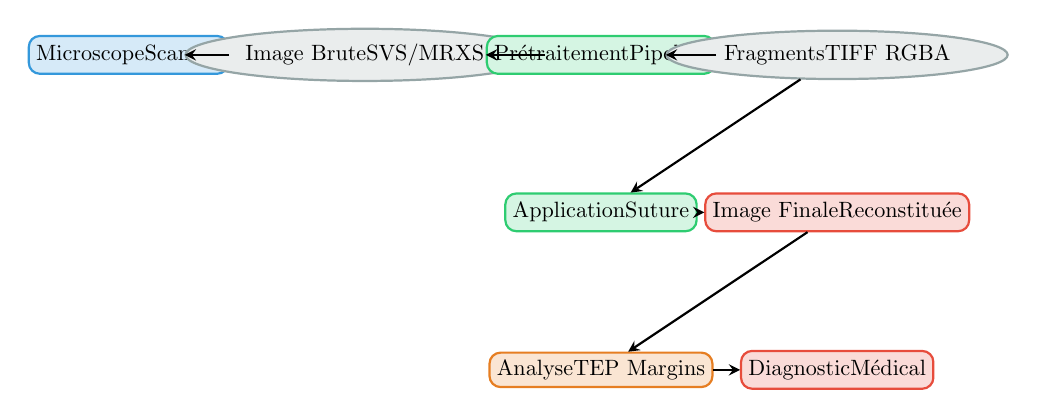
\begin{tikzpicture}[node distance=2cm, every node/.style={scale=0.8}]

% Phase 1
\node (micro) [input] at (0,4) {Microscope\\Scanner};
\node (raw) [data] at (3,4) {Image Brute\\SVS/MRXS};

% Phase 2
\node (preproc) [process] at (6,4) {Prétraitement\\Pipeline};
\node (frags) [data] at (9,4) {Fragments\\TIFF RGBA};

% Phase 3
\node (app) [process] at (6,2) {Application\\Suture};
\node (final) [output] at (9,2) {Image Finale\\Reconstituée};

% Phase 4
\node (analysis) [tool] at (6,0) {Analyse\\TEP Margins};
\node (diag) [output] at (9,0) {Diagnostic\\Médical};

% Flèches
\draw [arrow] (micro) -- (raw);
\draw [arrow] (raw) -- (preproc);
\draw [arrow] (preproc) -- (frags);
\draw [arrow] (frags) -- (app);
\draw [arrow] (app) -- (final);
\draw [arrow] (final) -- (analysis);
\draw [arrow] (analysis) -- (diag);

\end{tikzpicture}
\caption{Flux de données global du système}
\end{figure}

\chapter{Travail effectué}

\section{Module de prétraitement}

Le pipeline de prétraitement transforme les images brutes d'anatomopathologie en fragments exploitables. Cette étape automatisée combine l'expertise médicale (segmentation guidée) avec l'efficacité informatique.

% Schéma d'architecture du prétraitement
\begin{figure}[h!]
\centering
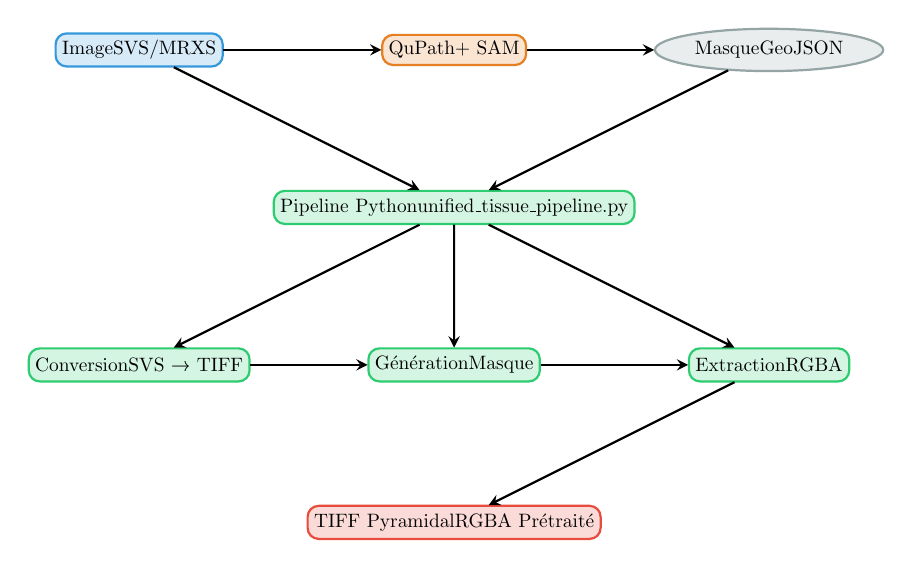
\begin{tikzpicture}[node distance=1.5cm, every node/.style={scale=0.7}]

% Ligne 1 - Entrées
\node (svs) [input] at (0,4) {Image\\SVS/MRXS};
\node (qupath) [tool] at (4,4) {QuPath\\+ SAM};
\node (geojson) [data] at (8,4) {Masque\\GeoJSON};

% Ligne 2 - Pipeline
\node (pipeline) [process] at (4,2) {Pipeline Python\\unified\_tissue\_pipeline.py};

% Ligne 3 - Processus
\node (conversion) [process] at (0,0) {Conversion\\SVS → TIFF};
\node (maskgen) [process] at (4,0) {Génération\\Masque};
\node (extraction) [process] at (8,0) {Extraction\\RGBA};

% Ligne 4 - Sortie
\node (tiffout) [output] at (4,-2) {TIFF Pyramidal\\RGBA Prétraité};

% Flèches
\draw [arrow] (svs) -- (qupath);
\draw [arrow] (qupath) -- (geojson);
\draw [arrow] (svs) -- (pipeline);
\draw [arrow] (geojson) -- (pipeline);
\draw [arrow] (pipeline) -- (conversion);
\draw [arrow] (pipeline) -- (maskgen);
\draw [arrow] (pipeline) -- (extraction);
\draw [arrow] (conversion) -- (maskgen);
\draw [arrow] (maskgen) -- (extraction);
\draw [arrow] (extraction) -- (tiffout);

\end{tikzpicture}
\caption{Architecture de la phase de prétraitement}
\end{figure}

% CAPTURE D'ÉCRAN : Pipeline en exécution
\begin{figure}[h!]
\centering
\includegraphics[width=0.8\textwidth]{images/pipeline_execution_screenshot.png}
\caption{Exécution de la pipeline de prétraitement}
\end{figure}

Le processus suit ces étapes principales :
\begin{enumerate}
\item \textbf{Segmentation avec QuPath} : Utilisation de QuPath enrichi du plugin SAM
\item \textbf{Export GeoJSON} : Sauvegarde des masques de segmentation
\item \textbf{Pipeline automatisé} : Traitement par le script \texttt{unified\_tissue\_pipeline.py}
\item \textbf{Génération TIFF RGBA} : Production de fichiers pyramidaux avec fond transparent
\end{enumerate}

\section{Module de suture interactive}

L'application de suture permet la manipulation manuelle des fragments prétraités pour reconstituer l'image histologique complète.

% Schéma d'architecture de l'application
\begin{figure}[h!]
\centering
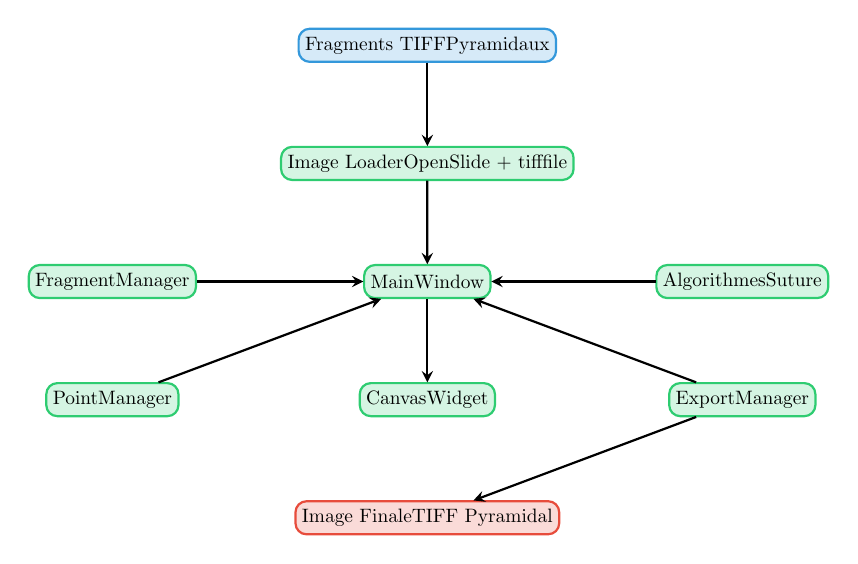
\begin{tikzpicture}[node distance=1.5cm, every node/.style={scale=0.7}]

% Entrée
\node (input) [input] at (4,6) {Fragments TIFF\\Pyramidaux};

% Chargement
\node (loader) [process] at (4,4.5) {Image Loader\\OpenSlide + tifffile};

% Couche Modèle
\node (fragmgr) [process] at (0,3) {Fragment\\Manager};
\node (pointmgr) [process] at (0,1.5) {Point\\Manager};

% Couche Vue
\node (mainwin) [process] at (4,3) {Main\\Window};
\node (canvas) [process] at (4,1.5) {Canvas\\Widget};

% Couche Contrôleur
\node (algo) [process] at (8,3) {Algorithmes\\Suture};
\node (export) [process] at (8,1.5) {Export\\Manager};

% Sortie
\node (output) [output] at (4,0) {Image Finale\\TIFF Pyramidal};

% Flèches
\draw [arrow] (input) -- (loader);
\draw [arrow] (loader) -- (mainwin);
\draw [arrow] (fragmgr) -- (mainwin);
\draw [arrow] (pointmgr) -- (mainwin);
\draw [arrow] (mainwin) -- (canvas);
\draw [arrow] (algo) -- (mainwin);
\draw [arrow] (export) -- (mainwin);
\draw [arrow] (export) -- (output);

\end{tikzpicture}
\caption{Architecture de l'application de suture}
\end{figure}

% CAPTURE D'ÉCRAN : Interface principale
\begin{figure}[h!]
\centering
\includegraphics[width=0.9\textwidth]{images/interface_principale_screenshot.png}
\caption{Interface principale de l'application}
\end{figure}

\subsection{Fonctionnalités principales}

L'application offre des outils complets de manipulation avec interface intuitive optimisée pour l'imagerie médicale.

% CAPTURE D'ÉCRAN : Canvas avec fragments
\begin{figure}[h!]
\centering
\includegraphics[width=0.8\textwidth]{images/canvas_fragments_screenshot.png}
\caption{Canvas de visualisation avec fragments}
\end{figure}

\subsubsection{Manipulation de groupe}

L'outil de sélection rectangle permet de manipuler plusieurs fragments simultanément.

\begin{figure}[h!]
\centering
\begin{subfigure}{0.48\textwidth}
\includegraphics[width=\textwidth]{images/selection_rectangle_screenshot.png}
\caption{Sélection rectangle}
\end{subfigure}
\hfill
\begin{subfigure}{0.48\textwidth}
\includegraphics[width=\textwidth]{images/panneau_groupe_screenshot.png}
\caption{Panneau de contrôle groupe}
\end{subfigure}
\caption{Système de sélection et manipulation de groupe}
\end{figure}

\subsubsection{Système de points étiquetés}

Cette fonctionnalité permet un alignement précis basé sur des correspondances définies manuellement.

\begin{figure}[h!]
\centering
\includegraphics[width=0.8\textwidth]{images/points_etiquetes_screenshot.png}
\caption{Système de points étiquetés pour alignement précis}
\end{figure}

\section{Exportation et formats de sortie}

L'interface d'exportation permet un contrôle précis des formats et niveaux de résolution.

\begin{figure}[h!]
\centering
\begin{subfigure}{0.48\textwidth}
\includegraphics[width=\textwidth]{images/dialogue_export_screenshot.png}
\caption{Dialogue d'exportation}
\end{subfigure}
\hfill
\begin{subfigure}{0.48\textwidth}
\includegraphics[width=\textwidth]{images/selection_niveaux_screenshot.png}
\caption{Sélection niveaux pyramidaux}
\end{subfigure}
\caption{Options d'exportation avancées}
\end{figure}

\subsection{Formats supportés}

L'application propose deux formats d'exportation principaux :

\begin{itemize}
\item \textbf{PNG} : Format standard pour visualisation et partage rapide
\item \textbf{TIFF pyramidal} : Préservation de la structure multi-résolution pour l'analyse approfondie
\end{itemize}

\section{Résultats et validation}

Les tests réalisés montrent une stabilité satisfaisante et des temps de réponse acceptables pour l'usage clinique. L'interface intuitive nécessite une formation minimale et s'intègre naturellement dans le processus existant.

\chapter{Conclusion}

\section{Bilan du stage}

Ce stage a permis de développer avec succès un outil complet de suture d'images histologiques répondant aux besoins spécifiques du projet TEP Margins. La solution développée combine efficacité technique et ergonomie d'utilisation, offrant aux laboratoires d'anatomopathologie un outil moderne pour la reconstruction d'images fragmentées.

\subsection{Objectifs atteints}

Les objectifs fixés en début de stage ont été entièrement réalisés :
\begin{itemize}
\item \textbf{Pipeline de prétraitement} : Fonctionnel et automatisé
\item \textbf{Interface de suture} : Complète avec toutes les fonctionnalités demandées
\item \textbf{Algorithmes d'alignement} : Deux approches complémentaires implémentées
\item \textbf{Export multi-format} : Support PNG et TIFF pyramidal
\end{itemize}

\section{Perspectives d'évolution}

L'outil développé constitue une base solide pour des évolutions futures. L'architecture modulaire facilite l'ajout de nouvelles fonctionnalités sans remise en cause de l'existant. Les perspectives incluent l'intégration d'intelligence artificielle pour l'alignement automatique, des fonctionnalités collaboratives, et une meilleure intégration avec les systèmes d'information hospitaliers.

\section{Conclusion générale}

Le développement de cet outil de suture d'images histologiques illustre parfaitement l'apport de l'informatique dans le domaine médical. En combinant expertise technique et compréhension des besoins cliniques, nous avons créé une solution sur mesure qui répond efficacement aux défis spécifiques du projet TEP Margins.

Cette expérience démontre l'importance de l'analyse approfondie des besoins et de la collaboration étroite avec les utilisateurs finaux pour développer des outils réellement adaptés aux contraintes du terrain médical.

\begin{thebibliography}{9}

\bibitem{openslide}
OpenSlide Contributors. \textit{OpenSlide: A vendor-neutral software foundation for digital pathology}. 
\url{https://openslide.org/}, 2023.

\bibitem{qupath}
Bankhead, P., Loughrey, M.B., Fernández, J.A. et al. 
\textit{QuPath: Open source software for digital pathology image analysis}. 
Scientific Reports 7, 16878 (2017).

\bibitem{sam}
Kirillov, A., Mintun, E., Ravi, N. et al. 
\textit{Segment Anything}. 
arXiv preprint arXiv:2304.02643 (2023).

\bibitem{ashlar}
Muhlich, J.L., Chen, Y.A., Yapp, C. et al. 
\textit{Stitching and registering highly multiplexed whole-slide images of tissues and tumors using ASHLAR}. 
Bioinformatics 38, 4613–4621 (2022).

\bibitem{pyqt6}
Riverbank Computing Limited. 
\textit{PyQt6 Reference Guide}. 
\url{https://doc.qt.io/qtforpython/}, 2023.

\bibitem{opencv}
Bradski, G. 
\textit{The OpenCV Library}. 
Dr. Dobb's Journal of Software Tools (2000).

\bibitem{tifffile}
Gohlke, C. 
\textit{Tifffile: Read and write TIFF files}. 
\url{https://github.com/cgohlke/tifffile}, 2023.

\bibitem{sift}
Lowe, D.G. 
\textit{Distinctive Image Features from Scale-Invariant Keypoints}. 
International Journal of Computer Vision 60, 91–110 (2004).

\bibitem{tepmargins}
Centre Henri Becquerel. 
\textit{Protocole TEP Margins - Évaluation des marges chirurgicales par micro-TEP}. 
Documentation interne, 2024.

\end{thebibliography}

\end{document}